%%%%%%%%%%%%%%%%%%%%%%%%%%%%%%%%%%%%%%%%%%%%%%%%%%%%%%%%%%%%%%%%%%%%%%%%%%%%%%%%
%                                                                              %
%	File:     sota.tex                                                         %
%   Document: XXX                                                              %
%   Author:   Freismuth David                                                  %
%	Date:	  22.JUN.2018                                                      %
%   Content:  Contains the State of the Art section of the Bachelor thesis.    %
%                                                                              %
%%%%%%%%%%%%%%%%%%%%%%%%%%%%%%%%%%%%%%%%%%%%%%%%%%%%%%%%%%%%%%%%%%%%%%%%%%%%%%%%

%%%%%%%%%%%%%%%%%%%%%%%%%%%%%%%%%%%%%%%%%%%%%%%%%%%%%%%%%%%%%%%%%%%%%%%%%%%%%%%%
\section{State of the Art}
Literature regarding this topic is very scarce, if not non-existent. At the timethis work has been released, no other publications, which attempted to establish 
an algorithm to automatically identify hardware designs, could be found.
Papers which worked on topics remotely relatable with the topic of hardware 
categorization, mostly presented methods to identify hardware trojans in a given 
design. This Hardware Trojan Identification can be seen as categorization into 
two groups: Non Hardware Trojan injected, and Hardware Trojan injected.
Identification of those Trojans is mostly achieved via a functional analysis [put sources here], where the design is simulated and tested for a certain
behaviour. Since our method aims for a structural analysis, these publications 
are hardly compareable to ours. Though one publication used a combination of structural- and 
functional analysis, to identify hardware trojan design patterns. This 
methodolodogy should be further looked upon.  

\subsection{Detection of Hardware Trojans}
In [literature] X net types are defined, which are typical for hardware trojans.
\label{hwTrojanNets} shows those proposed Hardware Trojans nets. Similar to 
our proposed method, the count of these nets are determined. 
 
\begin{figure}
    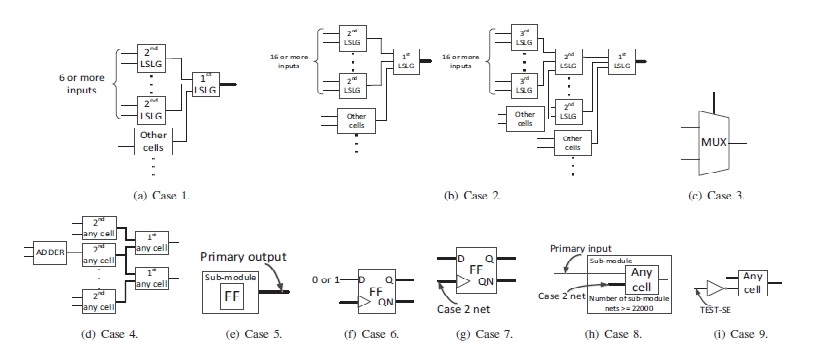
\includegraphics[width=\textwidth,keepaspectratio]{fig/hwTrojanNets.jpg}
    \label{hwTrojansNets}
    \caption{Register Transfer Level depiction of the proposed Hardware Trojan nets}
\end{figure}

The publication states, that trough the count of certain net types, the presence
of hardware trojans can be determined, but not their absence.
This insight leads to the assumption, that hardware design can be classified 
using the count of certain net types. 
